%% content.tex
%%


%% ===========================
\chapter{Umsetzung}
\label{ch:umsetzung}
%% ===========================

In diesem Kapitel wird auf die konkrete Umsetzung der Konzepte eingegangen. Die Komponenten des Systems selbst wurden aus architektonischer Sicht, wie in der Konzeption beschrieben umgesetzt. Daher wird vielmehr auf die genaue Umsetzung der Funktionen und Prozesse eingegangen. Anhand von Klassendiagrammen wird in den ersten beiden Kapiteln die Struktur und Funktionsweise der Webprojekte erläutert. Weiterhin wird der ETL-Prozess und die Abfrageerzeugung genauer betrachtet. Der genaue Ablauf in der Aktualisierung wird in dem darauf folgenden Abschnitt beschrieben. Abschließend wird der Aufbau der Oberfläche mit den damit verbundenen Designentscheidungen erläutert. 

%% ===========================
\section{Aufbau der Server.war}
%% ===========================

Die Web-Archive-Datei beinhaltet ein dynamisches Webprojekt aus dem Eclipse Web Tools Platform (WTP)-Projekt. Das Webprojekte besitzt die Struktur und Einstellungen die automatisch beim erzeugen des Projektes festgelegt werden. Deshalb wird direkt auf die Klassen eingegangen. Abbildung \ref{umsetzung_klassendiagramm_server} zeigt das Klassendiagramm der Server-WAR-Datei. Das Diagramm dient als Basis für die nachfolgenden Erläuterungen. 

Die H2-Datenbank wird im Embedded-Modus betrieben, was eine Instanziierung der Datenbank zur Laufzeit notwendig macht. Die Instanziierung erfolgt in der Klasse \textit{Database}. Das Attribut \textit{dataSource} stellt die H2-Datenbank in Form eines Objektes dar. Eine Verbindung zur Datenbank wird mithilfe der Methode \textit{getConnection()} aufgebaut. Diese Verbindung wird permanent offen gehalten, solang der Tomcat-Server läuft. Dazu wird die Verbindung dem Attribut \textit{con} zugewiesen, welches von allen Methoden verwendet wird, die eine Verbindung zur Datenbank aufbauen wollen. Um die Datenbank mit der Web-Anwendungen zu starten, ist die Verwendung eines Servlets nötig. Dazu benutzen wir die Klasse \textit{EntryPoint}, die das Interface \textit{HttpServlet} implementiert. Um das Servlet direkt beim Start aufzurufen sind in der \textit{web.xml} folgende Zeilen eingetragen: 

\begin{lstlisting}[language=XML]
	<servlet>
		<servlet-name>H2</servlet-name>
		<servlet-class>de.cas.db.EntryPoint</servlet-class>
		<load-on-startup>1</load-on-startup>
	</servlet>
\end{lstlisting}

Die 1 im Element \textit{<load-on-startup>} bewirkt den Aufruf der Methode \textit{init()} die eine Instanziierung der Klasse \textit{Database} vornimmt. Zur Erzeugung des Schemas wird eine separate Klasse namens \textit{SchemaBuilder} eingesetzt. In ihr werden sämtliche SQL-Anweisungen zur Generierung des Schemas aufbewahrt und können über die Methode \textit{createSchema()} ausgeführt werden.

\begin{figure}[htbp]
\begin{center}
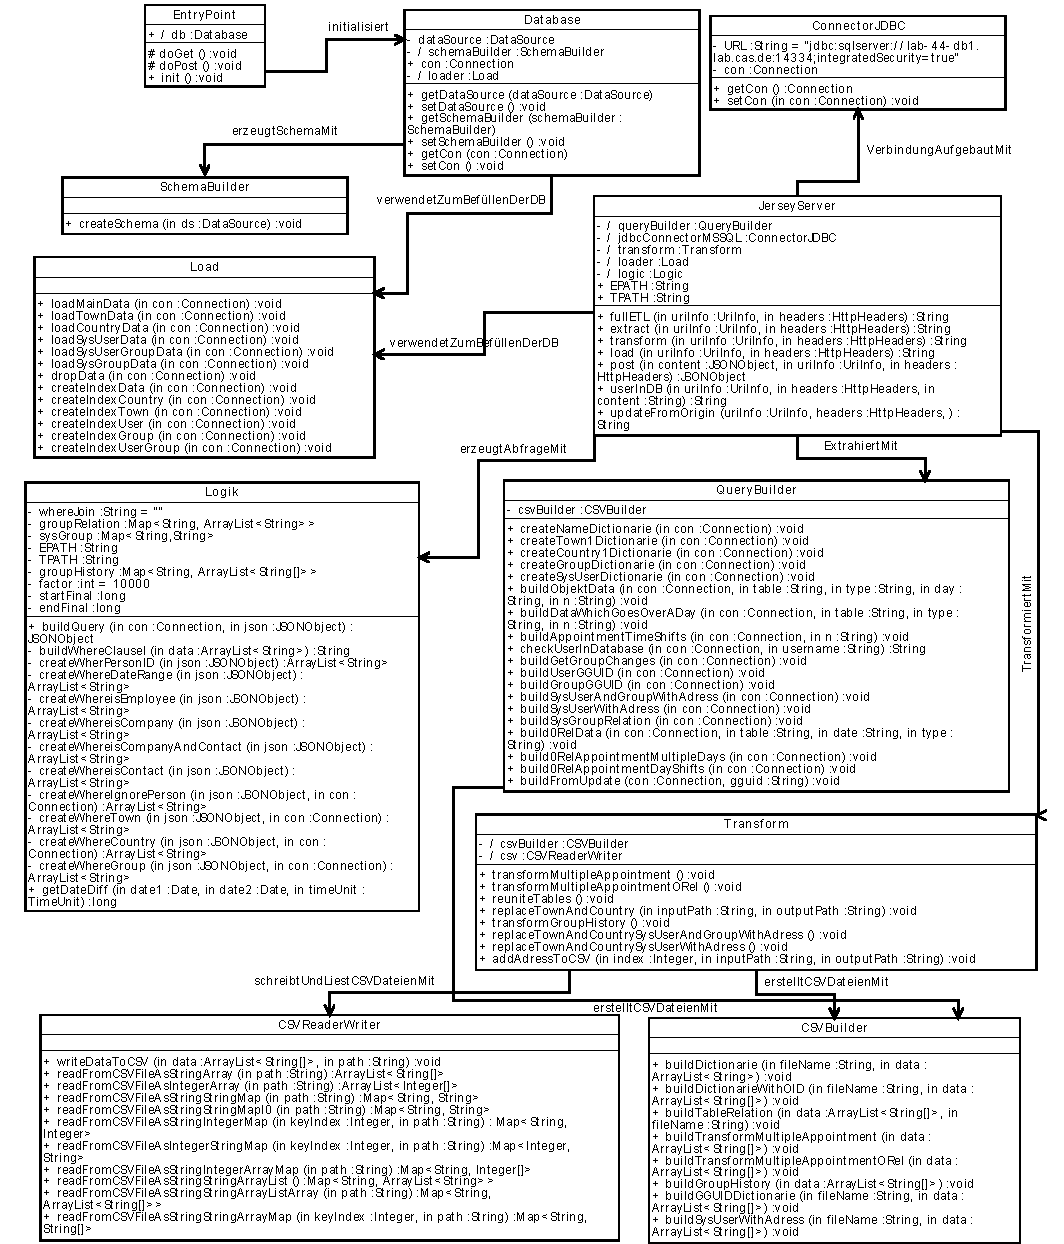
\includegraphics[width=1.0\textwidth]{pics/ServerKlassendiagramm.pdf}
\caption{Server Klassendiagramm}
\label{umsetzung_klassendiagramm_server}
\end{center}
\end{figure}

Mit der Klasse \textit{JerseyServer} wird der REST-Server umgesetzt. Sie besitzt Methoden die mit den entsprechenden Annotationen, wie \textit{@GET} oder \textit{@POST}, die REST-Requests entgegen nehmen. Mit der Annotation \textit{@Path} wird die URL angegeben, unter der die Methode angesprochen werden kann. Diese Methoden können Übergabeparameter vom Typ \textit{UriInfo} und/oder \textit{HttpHeaders} besitzen, die Abrufe von Metadaten der REST-Requests ermöglichen. 

Neben den Methoden zur Beantwortung von REST-Requests, enthält die Klasse alle Objekte zur Durchführung des ETL-Prozesses. Die Klasse \textit{ConnectorJDBC} besitzt ein Attribut namens \textit{con}, welches den Verbindungsaufbau zum MSSQL-Server, mithilfe von JDBC ermöglicht. Zur Extraktion der Daten aus dem MSSQL-Server wird ein Objekt der Klasse \textit{QueryBuilder} verwendet. Wie in der Abbildung zu sehen werden für die verschiedenen Tabellen, des neuen Schemas, eigene Methoden zur Verfügung gestellt. Methoden welche die Übergabewerte \textit{table}, \textit{date} und \textit{n} besitzen, werden für die verschiedenen Verbindungsmerkmale benötigt. Mithilfe des Parameters table wird der Name der Tabelle in der MSSQL Datenbank übergeben. Der Parameter \textit{date} gibt das Feld an, was für die Ermittlung des Datums verwendet werden soll. Um den Typ eines Verbindungsmerkmals zwischen Personen festzuhalten wird der Parameter \textit{n} verwendet, der eine Zahl zwischen eins und fünf beinhaltet. \textit{QueryBuilder} verwendet ein Objekt vom Typ \textit{CSV-Builder}, um die Ergebnisse in Dateien festzuhalten. Den Methoden wird als Übergabeparameter ein Dateiname, sowie die zu speichernden Informationen übergeben.

Die Klasse \textit{Transform} enthält Attribute und Methoden zur Bearbeitung der CSV-Dateien. Weiterhin werden die durch die Extraktionen gewonnen CSV-Dateien mithilfe eines \textit{CSVReaderWriter} Objekts ausgelesen. Nach der Bearbeitung durch die Methoden der \textit{Transform} Klasse, werden die Daten wieder in CSV-Dateien abgelegt. \textit{CSVBuilder} besitzt Methoden die zusätzliche Parameter zum schreiben aufweisen, die modifizierte Schreiboperationen erlauben. Wohingegen \textit{CSVReaderWriter} mithilfe der Methode \textit{writeDataToCSV()}, sowie den Parametern \textit{path} und \textit{data} allgemeine Schreiboperationen durchführt.

Mithilfe der Klasse \textit{Load} wird die Datenbank befüllt. Sie kann wie zuvor erwähnt von einem \textit{Database} Objekt verwendet werden oder durch ein \textit{JerseyServer} Objekt. Beim \textit{JerseyServer} werden mit der Methode \textit{load()} die Methoden der \textit{Load} Klasse aufgerufen. In der Klasse \textit{Database} werden sie im Konstruktor selbst aufgerufen. 

Die Klasse \textit{Logik} beinhaltet Attribute und Methoden zum beantworten von Benutzerabfragen. Um Bedingungen zu einer SQL-Abfrage hinzuzufügen werden separate Methoden verwendet. Die jeweiligen Methoden werden nur gerufen, sobald die entsprechende Bedingung in der vom Nutzer erhaltenen JSON-Datei vorhanden ist. Generiert werden die Abfragen durch die Methode \textit{buildQuery()}. 

%% ===========================
\section{Aufbau der Client.war}
\label{ch:Umsetzung:sec:clientwar}
%% ===========================

Einstiegspunkt in der Client.war ist die Klasse \textit{CasAnalyticUI}. Sie ist von der Klasse \textit{UI} abgeleitet. Die \textit{UI} ist die oberste Komponente jeder Komponentenhierarchie in Vaadin. Es gibt eine Benutzeroberfläche für jede Vaadin-Instanz in einem Browserfenster. Ein \textit{UI} Objekt kann entweder ein gesamtes Browserfenster(oder Tab) oder einen Teil einer HTML-Seite, wo eine Vaadin-Anwendung eingebettet ist darstellen. Nachdem eine \textit{UI} von der Anwendung erstellt wurde, wird diese mit der Methode \textit{init(VaadinRequest)} initialisiert. Zur Übersicht werden die Komponenten der Darstellung in die Klasse \textit{RootUI} ausgelagert. 

\textit{RootUI} wird dabei von der \textit{CasAnalayticUI} instanziiert. Die Klasse \textit{RootUI} beinhaltet das Anmeldefenster, sowie die Hauptansicht. Mithilfe der Methode buildLoginView() werden die Komponenten des Anmeldefensters zur \textit{UI} Komponente hinzugefügt. Nach der Erzeugung der Komponenten, wird eine \textit{JerseyClient} Klasse instanziiert. Diese wird verwendet sobald der Nutzer IP, Port und einen Namen eingegeben hat und auf anmelden klickt. Anschließend wird die Methode \textit{doPostRequestUserData()} gerufen, um zu überprüfen ob der Nutzer im System vorhanden ist. 

\begin{figure}[H]
\begin{center}
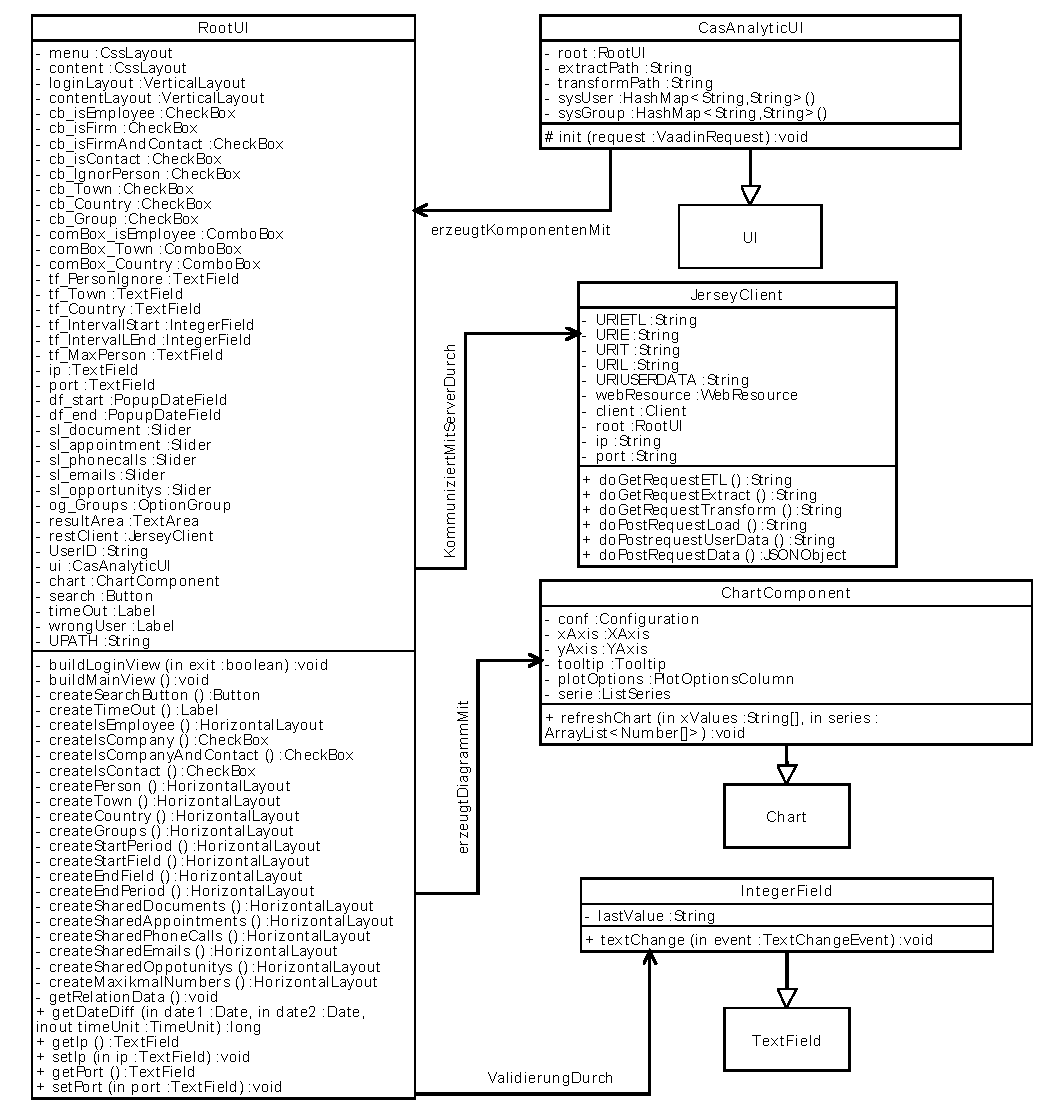
\includegraphics[width=1.0\textwidth]{pics/ClientKlassendiagramm.pdf}
\caption{Client Klassendiagramm}
\label{umsetzung_klassendiagramm_client}
\end{center}
\end{figure}

Falls ja, werden durch die Methode \textit{MainView()} alle bisherigen Komponenten der \textit{UI} entfernt und durch Komponenten des Hauptfensters ersetzt. Das \textit{JerseyClient} Objekt wird direkt im Anschluss verwendet, um Mithilfe der Methode \textit{doPostRequestData()} einen REST-Request an den Server zu senden. Dieser liefert das Ergebnis der Abfrage in einem JSON-Objekt zurück. Mit dessen eine erste Erzeugung des Diagramms durchgeführt wird. Das Diagramm selbst besitzt eine eigene Klasse namens \textit{ChartComponent}. Sie leitet sich von der Klasse \textit{Chart} ab, die Teil der VaadinChart-Bibliothek ist. Mithilfe der Methode \textit{refreshChart()} wird das Diagramm bei Benutzerabfragen aktualisiert. Dazu werden ihr die Namen der Personen für die x-Achse übergeben, sowie die neuen Balkenwerte. Weiterhin wird für jedes Vaadin-Objekt, welches eine Element an der Oberfläche darstellt, eine separate Methode zur Erzeugung verwendet. Änderungen am Aussehen oder an der Funktionalität der jeweiligen Vaadin-Objekte, werden nur innerhalb der entsprechenden Methode vorgenommen.

An der Oberfläche gibt es Felder die nur Zahlen erwarten. Eingaben die nicht numerisch sind werden durch den Einsatz der Klasse \textit{IntegerField} verhindert. Diese erweitert die Klasse \textit{TextField}. Sie besitzt einen Event-Listener, der jede Eingabe des Benutzers abfängt. Gibt der Nutzer nicht numerische Zeichen ein werden diese direkt wieder entfernt. Dadurch werden Falscheingaben durch den Nutzer ausgeschlossen.

%% ===========================
\section{Erzeugung der Abfrage}
%% ===========================

Um SQL-Abfragen möglichst schlank zu halten, erfolgt die Erzeugung dynamisch. Die SQL-Abfrage kann dadurch je nach Benutzereingabe unterschiedlich aufgebaut sein kann. Die Basisfunktionalität ändert sich allerdings nicht. Diese besteht aus der Bildung von Summen der verschiedenen Verbindungsmerkmale. Nachdem festgestellt wurde wie viele Verbindungsmerkmale von den jeweiligen Typen zu einer Person verlaufen, wird zusätzlich die Gesamtsumme der Verbindungsmerkmale zu einer Person gebildet. Die Summe wird zur Sortierung der Ergebnisse verwendet. Bei der Sortierung wird absteigend vorgegangen, um die Personen mit den meisten Verbindungsmerkmale zu der von der Suche ausgehend Person zu ermitteln. Das Ergebnis wird wiederum auf eine durch den Benutzer festgelegte Anzahl reduziert. Überdies beschränkt die Abfrage den Zeitraum durch die Verwendung der Spalte \textit{Date}.

Zu diesen Kernfunktionalitäten können durch Nutzerangaben weitere Funktionalitäten hinzukommen. Eine von ihnen stellt die Gewichtung von Zeitpunkten dar. Das Verfahren zur Gewichtung von Zeit wird anhand der Abbildung \ref{fig:umsetzung:gewichtungderzeit} erläutert. Die Abbildung zeigt ein Koordinatensystem mit der Gewichtung von einzelnen Zeitpunkten. Die x-Achse stellt den zeitlichen Verlauf und die y-Achse die Gewichtung dar. Der Startzeitpunkt wird durch $t_{s}$ markiert, wohingegen $t_{e}$ den Endzeitpunkt angibt. Mithilfe von $t_1$ und $t_2$ werden Zeitspannen festgelegt, die differenziert zu gewichten sind. Um nun die Tage zu gewichten wurde eine lineare Abstufung gewählt. Das bedeutet zwischen $t_{s}$ und $t_1$ steigt die Relevanz stetig, bis sie die 100\% erreicht hat. Ab dort besitzen alle Tage eine Relevanz von 100\%, außer es ist ein Wert für $t_2$ angegeben worden. Falls ja wird ab $t_2$ jeder Tag linear fallend bewertet. 

Um die Gewichtung zu einem bestimmten Tag zu berechnen werden die folgenden zwei Variablen verwenden:

\begin{equation}
f_1 = \frac{1}{t_1 - t_{s}}
\end{equation}
\begin{equation}
f_2 = \frac{1}{t_{e} - t_2}
\end{equation}


Dabei wird wie folgt vorgegangen. $t_{start}$ markiert den Ausgangszeitpunkt in Tagen. Aufsteigend zählend wird jeder Tag bis $t_1$ mit der Variabel $f_1$ multipliziert. Für den Zeitpunkt $t_2$ wird die Summe der Tage in der Zeitspanne zwischen $t_2$ und $t_{e}$ verwendet. Die Summe wird mit jedem weiteren Tag um 1 vermindert, bis zum Zeitpunkt $t_{e}$, der 0 darstellt. Bei jedem Schritt wird der Tag mit der Variablen $f_2$ multipliziert.

\begin{figure}[htbp]
\begin{center}
\begin{tikzpicture}[domain=-1:2] \draw[very thin,color=gray] (0,0); 
\draw[->] (0,0) -- (12.3,0) node[right] {Zeit}; 
\draw[->] (0,0) -- (0,4.2) node[above] {Faktor Gewichtung}; 
\draw[color=black]  (0.2,3) -- (-0.2,3)   node[left] {100\%};
\draw[color=black]  (0.2,1.5) -- (-0.2,1.5)   node[left] {50\%};  
%\draw[dashed][color=black]  (4,0.5) -- (4,3.5); 
%\draw[dashed][color=black]  (9,0.5) -- (9,3.5);

\draw[color=black]  (0,0) -- (0,0)   node[below] {$t_{s}$}; 
\draw[color=black]  (4,0.1) -- (4,-0.1)   node[below] {$t_1$}; 
\draw[color=black]  (9,0.1) -- (9,-0.1)   node[below] {$t_2$};
\draw[color=black]  (12,0.1) -- (12,-0.1)   node[below] {$t_{e}$};   
 
\draw[color=black]  (0,0) -- (4,3)   node[right] {}; 
\draw[color=black]  (4,3) -- (9,3)   node[right] {}; 
\draw[color=black]  (9,3) -- (12,0)   node[right] {};  

\draw[dotted][color=black]  (0.5,0.75) -- (1.5,0.75);
\draw[dotted][color=black]  (1.5,1.5) -- (2.5,1.5);
\draw[dotted][color=black]  (2.5,2.25) -- (3.5,2.25);
\draw[dotted][color=black]  (3.5,3) -- (4.5,3);

\draw[dotted][color=black]  (0.5,0.75) -- (0.5,0);
\draw[dotted][color=black]  (1.5,1.5) -- (1.5,0);
\draw[dotted][color=black]  (2.5,2.25) -- (2.5,0);
\draw[dotted][color=black]  (3.5,3) -- (3.5,0);
\draw[dotted][color=black]  (4.5,3) -- (4.5,0);

\draw[dotted][color=black]  (8.5,3) -- (8.5,0);
\draw[dotted][color=black]  (9.5,3) -- (9.5,0);
\draw[dotted][color=black]  (10.5,2) -- (10.5,0);
\draw[dotted][color=black]  (11.5,1) -- (11.5,0);

\draw[dotted][color=black]  (8.5,3) -- (9.5,3);
\draw[dotted][color=black]  (9.5,2) -- (10.5,2);
\draw[dotted][color=black]  (10.5,1) -- (11.5,1);

\draw[dotted][color=black]  (1,0.75) -- (1,1.05)   node[above] {$t_{s}+1$}; 
\draw[dotted][color=black]  (2,1.5) -- (2,1.8)   node[above] {$t_{s}+2$}; 
\draw[dotted][color=black]  (3,2.25) -- (3,2.55)   node[above] {$t_{s}+3$}; 
\draw[dotted][color=black]  (4,3) -- (4,3.3)   node[above] {$t_{s}+4$}; 

\draw[dotted][color=black]  (9,3) -- (9,3.3)   node[above] {$t_{e}-3$}; 
\draw[dotted][color=black]  (10,2) -- (10,2.3)   node[above] {$t_{e}-2$}; 
\draw[dotted][color=black]  (11,1) -- (11,1.3)   node[above] {$t_{e}-1$}; 

\end{tikzpicture} 
\end{center}
\caption{Gewichtung der Zeit}
\label{fig:umsetzung:gewichtungderzeit}
\end{figure}

Neben der Gewichtung der Zeit lassen sich die jeweiligen Verbindungsmerkmale unterschiedlich gewichten. Bei einer Abweichung von 100 Prozent wird die Summe des jeweiligen Verbindungsmerkmales, um die durch den Nutzer bestimmten Prozentsatz verringert. 

Die restlichen Parameter filtern die SQL-Abfrage und werden nach Bedarf hinzugezogen. Eine der Konditionen muss zuvor ermittelt werden und wird daher näher beschrieben. Es handelt sich dabei um Gruppen, die aus der Ergebnismenge ausgeschlossen werden können. Ihre Struktur ist im Laufe der Zeit variabel. Um dies zu berücksichtigen wird die Tabelle \textit{UserGroup} verwendet. Dabei folgendermaßen vorgegangen: Zuerst wird die Ergebnismenge durch die ausgewählten Gruppen reduziert. Anschließend wird für jede Gruppe ein eigener Container erzeugt. Der Container beinhaltet die ID der Personen aus der Gruppe. Liegt nun der Zeitpunkt des Feldes \textit{Date} nach dem Anfangszeitpunkt der Abfrage und die Spalte \textit{Action} enthält eine 1, wird der Container um diese Person reduziert. Enthält sie eine 0, wird die Person zum Container hinzugefügt. Mit einer 1 in der Spalte \textit{Action} wird der Austritt einer Person aus der Gruppe markiert. Eine 0 weist auf den Eintritt einer Person in die Gruppe hin. Dadurch wird die Struktur der Gruppe zum Anfangszeitpunkt wiederhergestellt. Mithilfe der Personen aus den Container, wird nun die SQL-Abfrage um weitere Bedingungen erweitert.

Innerhalb von Zeiträumen können sich Gruppen verändern, jedoch können diese nicht berücksichtigt werden. Es kann jeweils nur ein bestimmter Zeitpunkt betrachtet werden. In unserem Fall entschied man sich für den Anfangszeitpunkt $t_{s}$.

%% ===========================
\section{ETL Prozess}
%% ===========================

Um an die notwendigen Daten zu gelangen werden zuerst die Informationen aus der MSSQL-Datenbank extrahiert. Dazu wird ein Verbund gebildet, der Tupeln aus den betroffenen Tabellen verschmelzen lässt. Die in CAS genesisWorld manuell hinterlegten Verbindungen werden mithilfe der Tabelle \textit{TableRelation} ermittelt. Zur Beschaffung der Verbindungen wird als erstes eine SQL-Abfrage definiert, die für jede der Tabellen \textit{gwOpportunity}, \textit{gwPhoneCall0}, \textit{Document0}, \textit{EmailStore0} und \textit{Appointment0} separat ausgeführt wird. 

Mithilfe eines Verbundes zwischen den Tabellen \textit{SysUser} und \textit{Address0} werden die Adressen zu den Personen ermittelt. Anschließend werden durch einen Verbund zwischen \textit{TableRelation} und \textit{SysUser} alle Tabellen ermittelt die mit den Personen eine Verbindung besitzen. Der nächste Verbund wird zwischen \textit{TableRealtion} und einer der fünf zuvor genannten Tabellen gebildet. Um beispielsweise festzustellen welche anderen Personen mit einem Dokument arbeiten, wird ein weiterer Verbund mit der passenden ORel-Tabelle gebildet. In der ORel-Tabelle kann die \textit{OID} positiv, sowie negativ sein. Bei einem negativen Wert stellt die \textit{OID}, eine \textit{GID} der Tabelle \textit{SysGroup} dar. Zur Auflösung von Gruppen in einzelne Personen werden folgende Verbunde gebildet. Zuerst zwischen \textit{SysGroup} und \textit{SysGroupMember}, um alle Personen die zu einer Gruppe gehören zu erhalten. Anschließend zwischen \textit{SysGroupMember} und \textit{SysUser}, um die \textit{OID} der Person zu erhalten. 


Die durch den Verbund gewonnen Informationen werden weiterhin auf drei relevante Werte verringert. Zu einem die \textit{OID} des \textit{SysUser}, von dem die Suche ausgeht. Zum anderen das Datum, welches durch ein Verbindungsmerkmal ermittelt wird. Weiterhin wird die zweite \textit{OID} behalten, die durch den Verbund mit einer zweiten \textit{SysUser} Tabelle gewonnen wird. Zum Schluss wird manuell eine vierte Information beigefügt, die besagt welchem Verbindungsmerkmal die Tupel entstammt. 

Für den Sonderfall das ein Datum über mehrere Tage geht, wird eine fünfte Spalte hinzugefügt, welche den Zeitraum in Tagen beinhaltet. Zur Beschaffung der geschobenen Termine wird genau wie in der Konzeption beschrieben verfahren.

Zur Ermittlung von direkten Verbindungen zwischen Personen wird lediglich ein Verbund aus den ORel-Tabellen eines Verbindungsmerkmales gebildet. Dieser Verbund beinhaltet bereits die \textit{OID} der beiden Personen. Zur Ermittlung des Datums wird noch ein Verbund mit der Tabelle des Verbindungsmerkmals gebildet. Die negativen \textit{OID} Werte werden genauso wie oben beschrieben aufgelöst. 

Jedes Ergebnis einer Extraktionsabfrage wird in einer CSV-Datei direkt auf dem Tomcat gespeichert. Diese CSV-Dateien stellen die Grundlage der Transformation dar. Jede dieser Dateien beinhaltet Verbindungen zwischen Personen, in der Form wie sie in Abbildung \ref{fig:umsetzung_csv_datei} zu sehen ist. 

\begin{figure}[htbp]
\begin{center}
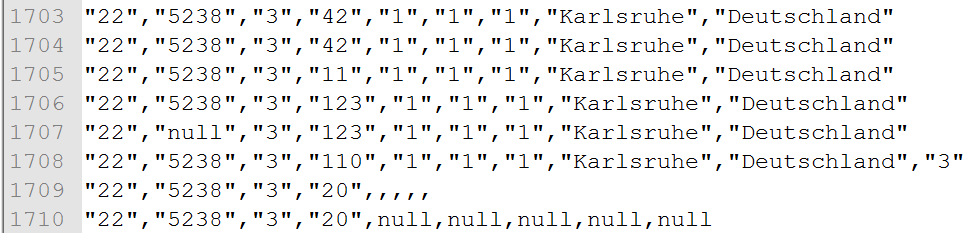
\includegraphics[width=1.0\textwidth]{pics/umsetzung_csv_datei.png}
\caption{Ausschnitt einer CSV-Datei nach der Extraktion}
\label{fig:umsetzung_csv_datei}
\end{center}
\end{figure}

Alle CSV-Dateien werden auf die in Abbildung \ref{fig:umsetzung_csv_datei} zu sehenden Ungereimtheiten untersucht. Dabei wird in Zeilen in denen die letzten fünf Werte fehlen, die Adresse über die \textit{OID} (die vierte Zahl) ergänzt. Bei Nullwerten wird überprüft ob wirklich keine Adresse vorhanden ist, falls doch werden die Adressen ergänzt. Wenn wie in Zeile 1707 zu sehen, ein Nullwert anstatt eines Datum existiert, wird die Zeile entfernt. Wenn wie in Zeile 1708 ein zusätzlicher Wert vorhanden ist, erstreckt sich das Merkmal über mehrere Tage. Die Zeile bleibt bestehen allerdings wird der letzte Wert entfernt. Die Zahl wird jedoch zwischengespeichert, um die entsprechende Anzahl an Tupeln zu erzeugen. Jede dieser Tupeln weist auf einen anderen Tag in der Zeitspanne hin. Nach der Beseitigung von Anomalien werden noch die Städte und Länder durch ihre jeweilige \textit{ID} aus der Tabelle \textit{Town} und \textit{Country} ersetzt.

Die veränderten Daten werden wieder in CSV-Dateien abgelegt. Diese besitzen den gleichen Namen, besitzen allerdings noch den Zusatz "\_transf", der sie als transformiert kennzeichnet. Diese Dateien werden anschließend in einer CSV-Datei zusammengeführt. Bei der Zusammenführung sind zum ersten mal alle Daten gleichzeitig in der Anwendung vorhanden, weshalb an dieser Stelle alle Duplikate beseitigt werden. Weiterhin werden überdies die Zeilen sortiert. Dabei wird mit zwei Kriterien verfahren. Das erste Kriterium ist die \textit{OID} der Person von der die Suche ausgeht. Falls Werte sich gleichen wird das zweite Feld (Datum) herangezogen. Nachdem alle Zeilen sortiert und von Duplikaten bereinigt sind, werden sie in einer CSV-Datei abgelegt. 

Diese Datei werden bei jedem Start der Datenbank verwendet, um einen Bulk-Load für die H2-Datenbank zu initialisieren. Nach dem Einfügen der Daten in die Datenbank werden die Indizes auf den Datensätzen erzeugt.


%% ===========================
\section{Aktualisierung des Datenbestandes}
%% ===========================

Wie zuvor in Abschnitt \ref{ch:Konzeption:sec:updatedatenbestand} behandelt, wird die Aktualisierung unseres Datenbestandes von CAS genesisWorld angestoßen. Die Implementierung ist in Form einer COM-Komponente umgesetzt. Sie wird in einer DLL-Datei definiert. Diese muss Namenskonventionen einhalten. Es werden nur Dateien vom CAS genesisWorld Anwendungsserver erkannt die mit dem Prefix \textit{pGSAxExtCustomServerDataPlugin} beginnen. Die DLL-Datei ist in der \textit{RegisterSDKDataPlugIns.xml} hinterlegt, damit der Anwendungsserver beim Start das Plugin findet. Weiterhin ist in der XML-Datei eine Tabelle paarweise mit einer DLL angegeben. Dadurch wird ein Plugin auf eine Datenbanktabelle registriert und bekommt alle betreffenden Änderungen mit.

\begin{figure}[htbp]
\centering
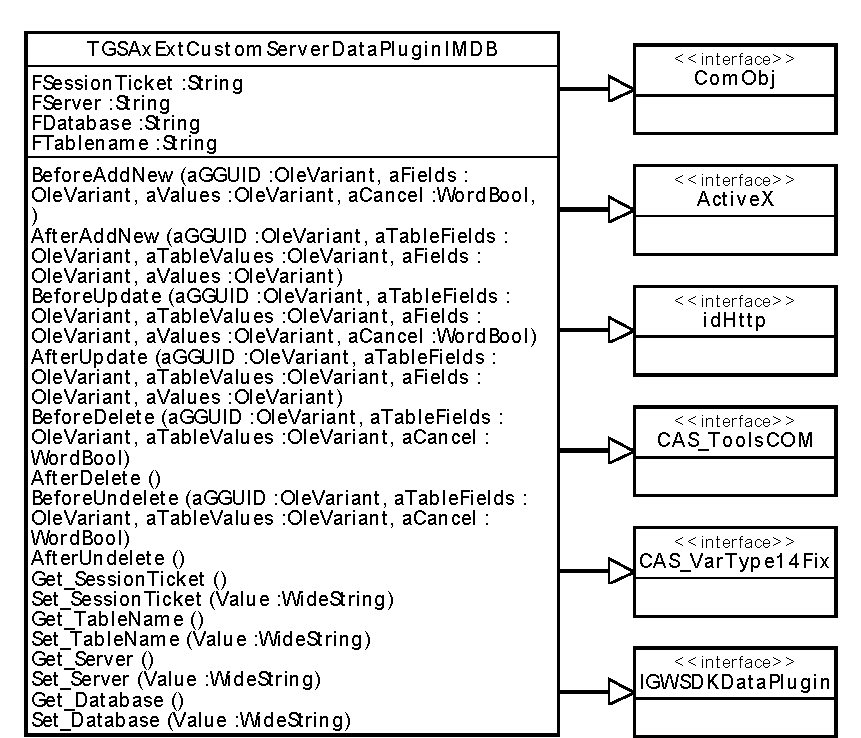
\includegraphics[scale=0.8]{pics/plugin_klassendiagramm.pdf}
\caption{Klassendiagramm Plugin}
\label{ergebniss_plugin_klassendiagramm}
\end{figure}

Die Programmbibliothek selbst ist in Delphi geschrieben. Abbildung \ref{ergebniss_plugin_klassendiagramm} zeigt die Struktur der DLL-Datei. Die Klasse selbst implementiert sechs verschiedene Schnittstellen. \textit{ComObj} stellt Funktionen zur Erstellung und Bearbeitung von COM-Objekten zur Verfügung. Um Funktionalitäten von CAS genesisWorld vollständig zu nutzen, wird die \textit{ActiveX} Schnittstelle benötigt. Wie bereits behandelt findet die Übertragung der Daten über das REST-Protokoll statt, wofür die \textit{idHttp} Schnittstelle verwendet wird. Um Konvertierungen der vom Anwendungsserver erhaltenen Binärwerte vorzunehmen, werden die Funktionen der Schnittstellen \textit{CAS\_ToolsCOM} und \textit{CAS\_VarType14Fix} genutzt. Das Abfangen der geänderten Daten, welches die eigentliche Kernfunktionalität darstellt, wird durch die Funktionen der \textit{IGWSDKDataPlugin} Schnittstelle implementiert.

Die Funktionen der Abbildung \ref{ergebniss_plugin_klassendiagramm} gehören von \textit{BeforeAddNew()} bis \textit{AfterUndelete()} zur \textit{IGWSDKDataPlugin} Schnittstelle. Es sind zwar alle Funktionen der \textit{IGWSDKDataPlugin} Schnittstelle in der DLL implementiert, allerdings sind nur die Funktionen die mit \textit{After} beginnen auch mit Logik hinterlegt. Für unser System reicht es nämlich aus, über Änderungen im Nachhinein benachrichtigt zu werden. Die Funktionen enthalten alle die gleiche Logik und unterscheiden sich lediglich in den Übergabeparameter.

Die Funktionsweise wird im Folgenden anhand der Abläufe in der Logik erläutert. Nachdem der Nutzer Datensätze geändert hat wird das Plugin aufgerufen. Die entsprechende Funktion erhält die \textit{GGUID} der Tupel, den Namen der Spalte, sowie die veränderten Werte. Anschließend wird überprüft, ob die Änderungen für unser System von Relevanz ist. Falls sie sich als relevant herausstellen, wird die \textit{aGGUID} in einen String konvertiert. Anschließend werden die Header-Werte der \textit{idHttp} Variable gesetzt. Sie beinhalten Werte wie die URI oder HTTP-Metadaten. Sobald alle Daten in der \textit{idHttp} gesetzt sind, wird ein POST-Request an unser System übermittelt. 

Der POST-Request enthält lediglich die \textit{GGUID} und die Art der Operation, die auf den Daten ausgeführt wurde. Bei neuen Daten beispielsweise wird ein Header namens "newGGUID" und dem Wert der \textit{GGUID} gesetzt. Im Anwendungsserver wird der neue Wert zuerst in eine CSV-Datei geschrieben und anschließend in die Datenbank eingefügt.


%% ===========================
\section{Oberfläche}
%% ===========================

In diesem Abschnitt wird die Umsetzung der Darstellung erörtert. Den Einstiegspunkt für Nutzer stellt das in Abbildung \ref{ergebniss_oberflaeche_anmeld} zu sehende Anmeldefenster dar. Der Hintergrund der Webseite ist in einem dunklen grau gestaltet, um einen Kontrast zum weißen Hintergrund der Bedienelemente zu schaffen. Dadurch werden die für den Nutzer verwendbaren Bereiche abgehoben. Zur Identifikation des Systems mit der Firma ist das Logo der CAS Software AG im linken Teil abgebildet. Im rechten Teil des Fensters existieren drei Eingabefelder. Zuerst ein Feld zur Eingabe der IP-Adresse des Server. Die dazugehörige Portnummer wird im darauf folgenden Feld eingegeben. Das dritte Feld ist für den Namen des Nutzers vorgesehen, der den Ausgangspunkt der Analyse darstellt. Abschließend wird ganz klassisch ein Button zum fortfahren auf der Webseite eingesetzt. Falls allerdings der eingegeben Nutzername nicht existiert, wird eine Warnmeldung direkt über dem zweiten Eingabefeld ausgegeben. 

\begin{figure}[htbp]
\centering
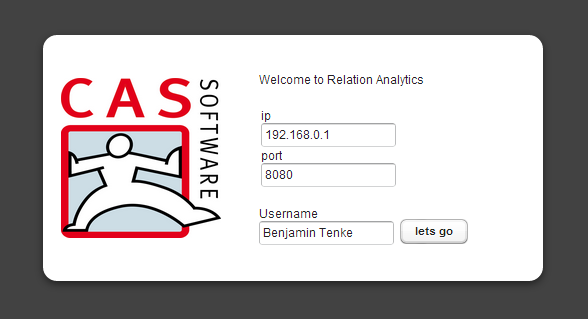
\includegraphics[scale=2.0]{pics/login.png}
\caption{Anmeldefenster}
\label{ergebniss_oberflaeche_anmeld}
\end{figure}

Das Hauptfenster wurde vom Aufbau, wie in Abschnitt \ref{ch:Konzeption:sec:Darstellungskonzepte} beschrieben umgesetzt. Im oberen Bereich befindet sich eine Leiste, die anhand der Microsoft Richtlinien für Design entworfen wurde. Dies schafft ein vertrautes Gefühl mit der Oberfläche und schafft eine schnelle Akzeptanz bei den Nutzern. Die Leiste ist in vier Bereiche aufgeteilt. Der erste Bereich, ganz links, dient der Gewichtung der Verbindungsmerkmale und dem anstoßen der Abfrage. Aufgrund der Gewichtung in Prozent, ist ein fester Wertebereich von 0 bis 100 vorgegeben. Textfelder eignen sich daher weniger, da sie beliebige Eingaben ermöglichen. Der Einsatz von Reglern bietet eine einfachere und selbsterklärende Form der Bedienung. Der begrenzte sowie kleine Wertebereich führte zu dieser Entscheidung. Zum stellen der Anfrage wird ein einfacher Button eingesetzt. Direkt unter dem Button befindet sich ein Text, der die benötigten Zeit für die Abfrage ausgibt. 

Der zweite Bereich dient zeitlichen Anpassungen. Das erste und dritte Feld können für Veränderung des Betrachtungszeitraums verwendet werden. Sie beinhalten den Anfangs- und Endzeitpunkt. Händische Eingaben weisen eine schlechte Bedienbarkeit auf, weswegen ein sogenannter "Datumspicker" eingesetzt wird. Dieser befindet sich direkt neben dem Textfeld und öffnet sich nach einem Klick auf das Symbol. Er stellt einen grafischen Kalender dar, aus dem durch klicken auf ein Tag, das Datum bestimmt werden kann. Die Möglichkeit zur Eingabe durch direktes ändern des Textes bleibt allerdings weiterhin erhalten. Die anderen beiden Felder sind für die Gewichtung der Zeit vorgesehen. Diese Felder dienen zur Festlegung von $t_1$ und $t_2$, aus der Abbildung \ref{fig:umsetzung:gewichtungderzeit}. Das obere Feld ist für $t_1$. Hier kann die Zeitspanne zwischen $t_{s}$ und $t_1$ in Tagen festgelegt werden. Für $t_{e}$ und $t_2$ verhehlt es sich wie mit dem unteren Feld.

Bis auf die Gruppenfilterung sind im dritten Bereich alle restlichen Filtermöglichkeiten vorhanden. Mithilfe von Checkboxen kann der Nutzer festlegen, welche Filterungen auf die Analyse angewendet werden sollten. Neben der Filterung durch bestimmte Personen, Länder, Städte usw. ist hier eine Begrenzung der Ergebnismenge umgesetzt. Im untersten Feld kann der Nutzer diese bestimmen.

Der Bereich ganz rechts in der Leiste, ist für den Ausschluss von Gruppen vorgesehen. Hier werden alle Gruppen im System mit einer Checkbox und einem Namen dargestellt. Dabei können beliebig viele Gruppen ausgewählt werden. Da die Anzahl der Gruppen überschaubar ist, entschied man sich alle anzuzeigen, anstatt einer händischen Eingabe der Namen durch den Nutzer. Für Benutzer entsteht dadurch ein Vorteil, da sie Gruppen auswählen können die sie zuvor nicht kannten.

\begin{figure}[htbp]
\centering
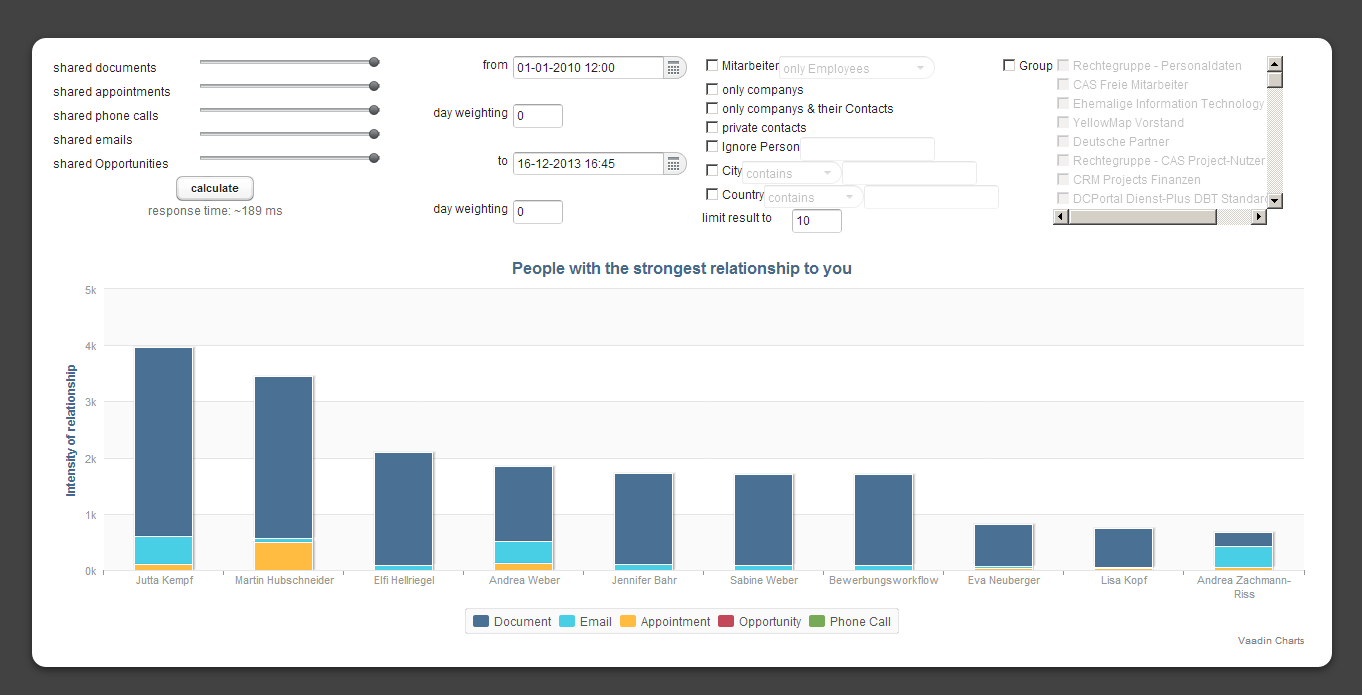
\includegraphics[width=\textwidth]{pics/final_screen.png}
\caption{Hauptseite der Anwendung}
\label{ergebniss_oberflaeche_haupt}
\end{figure}

Den zentralen Bereich des Fensters stellt das Diagramm dar. Die Balken selbst sind in fünf verschiedene Elemente unterteilt. Jedes Elemente wird dabei, durch eine andere Farbe dargestellt. Die fünf Elemente sind die verschiedenen Verbindungsmerkmale. Die Zuordnung der Farbe zu dem jeweiligen Merkmal, wird über eine Legende im unteren Bereich des Fensters umgesetzt. Eine Besonderheit ist, dass durch einen Klick auf eine der Farben, das jeweilige Merkmal von der Darstellung ausgeschlossen wird. Beispielsweise kann der Nutzer auf die blaue Farbe neben dem Dokument klicken, was einen Neuaufbau des Diagramms ohne Dokumente bewirkt. Durch den Ausschluss wird allerdings keine neue Abfrage gesendet. Das  bedeutet die Reihenfolge in der die Personen angezeigt werden die Datenbasis gleich  bleiben. Mit einem wiederholten Klick lässt sich der Originalzustand wiederherstellen. Zusätzlich zu der y-Achse, die eine Gesamtpunktzahl aufzeigt, kann der jeweilige Anteil eines Merkmals betrachtet werden. Dies geschieht durch einfaches platzieren des Mauszeigers, auf dem jeweiligen Bereich des Balkens. Dadurch öffnet sich ein Tooltip, welches die Anzahl der Punkte im Verhältnis zur Gesamtpunktzahl zeigt.

Die Ausführung der Anfrage erfolgt in der Regel mit dem dafür vorgesehen Button. Die Regler und das Datum, jedoch lösen bei Veränderungen automatisch eine neue Abfrage aus. Dies soll die hohe Antwortgeschwindigkeit des Systems untermalen und eine bessere Nutzererfahrung schaffen. Das Datum, sowie die Gewichtung wurden dazu ausgewählt, da sie die am meisten benutze Konfigurationsmöglichkeit darstellen.